%%%%%%%%%%%%%%%%%%%%%%%%%%%%%%%%%%%%%%%%%
% Engineering Calculation Paper
% LaTeX Template
% Version 1.0 (20/1/13)
%
% This template has been downloaded from:
% http://www.LaTeXTemplates.com
%
% Original author:
% Dmitry Volynkin (dim_voly@yahoo.com.au)
%
% License:
% CC BY-NC-SA 3.0 (http://creativecommons.org/licenses/by-nc-sa/3.0/)
%
%%%%%%%%%%%%%%%%%%%%%%%%%%%%%%%%%%%%%%%%%

%----------------------------------------------------------------------------------------
%	PACKAGES AND OTHER DOCUMENT CONFIGURATIONS
%----------------------------------------------------------------------------------------

\documentclass[12pt,a4paper]{article} % Use A4 paper with a 12pt font size - different paper sizes will require manual recalculation of page margins and border positions
\usepackage[utf8]{inputenc}
\usepackage{marginnote} % Required for margin notes
\usepackage{wallpaper} % Required to set each page to have a background
\usepackage[francais]{babel}
%\usepackage{bclogo}
\usepackage{tikz}
\usetikzlibrary{shapes,snakes}
\usetikzlibrary{mindmap,trees}
\usepackage{lastpage} % Required to print the total number of pages
\usepackage[left=1.3cm,right=4.6cm,top=1.8cm,bottom=4.0cm,marginparwidth=3.4cm]{geometry} % Adjust page margins
\usepackage{amsmath} % Required for equation customization
\usepackage{amssymb} % Required to include mathematical symbols
\usepackage{xcolor} % Required to specify colors by name
\usepackage{enumerate}


\usepackage{tikz}
\usepackage[most]{tcolorbox}
\usepackage[pstricks]{bclogo}
\usepackage{pst-blur}

\usepackage{fancyhdr} % Required to customize headers
\setlength{\headheight}{80pt} % Increase the size of the header to accommodate meta-information
\pagestyle{fancy}\fancyhf{} % Use the custom header specified below
\renewcommand{\headrulewidth}{0pt} % Remove the default horizontal rule under the header

\setlength{\parindent}{0cm} % Remove paragraph indentation
\newcommand{\tab}{\hspace*{2em}} % Defines a new command for some horizontal space


%%%%%%%%%
%\renewcommand{\thesubsection}{[\Alph{section}](\alph{subsection})}
%%%%%%%%%

\newcommand\BackgroundStructure{ % Command to specify the background of each page
\setlength{\unitlength}{1mm} % Set the unit length to millimeters

\setlength\fboxsep{0mm} % Adjusts the distance between the frameboxes and the borderlines
\setlength\fboxrule{0.5mm} % Increase the thickness of the border line
\put(10, 10){\fcolorbox{black}{blue!1}{\framebox(155,247){}}} % Blue!1 , le numéro change la l'opacité de la couleur bleu
\put(165, 10){\fcolorbox{black}{blue!10}{\framebox(37,247){}}} % Margin box
\put(10, 262){\fcolorbox{black}{white!10}{\framebox(192, 25){}}} % Header box 160 et 263 pour régler la position du logo
\put(178, 263)    {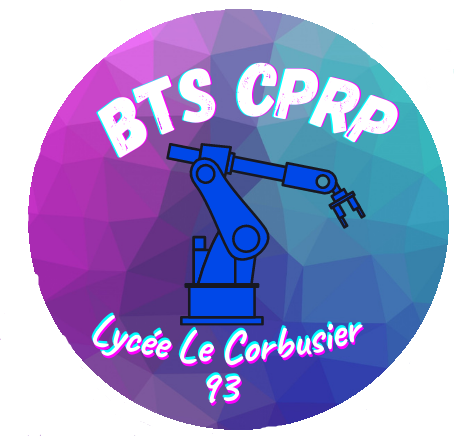
\includegraphics[height=23mm,keepaspectratio]{logo.png}} % Logo box - maximum height/width: 
}






%----------------------------------------------------------------------------------------
%	HEADER INFORMATION
%----------------------------------------------------------------------------------------
\fancyhead[L]{\begin{center}\textbf{\textcolor{red}{CORRECTION}}\end{center} 
\begin{tabular}{l r | l r} 
\textbf{Sujet} & TP2.1 Désignation des outils de production  & TP noté $1^{er}$ semestre \\ 
\textbf{BTS} & CPRP 1 & \the\year-2023 & Page : \thepage/\pageref{LastPage} \\ 
\end{tabular}}
%----------------------------------------------------------------------------------------










\begin{document}


%%%%POUR FAIRE DES EXERCICES INDÉPENDAMMENT DES SECTIONS%%%%
%%%%%%%%%%%%%%%%%%%%%%%%%%%%%%%%%%%%%%%%%%%%%%%%%%%%%%%%%%%%%%%%%%%
\newcounter{exo}
\newenvironment{exo}{\stepcounter{exo}\vspace{0.5cm}{\bfseries Question \theexo\ :}}{\par\vspace{0.5cm}}
%%%%%%%%%%%%%%%%%%%%%%%%%%%%%%%%%%%%%%%%%%%%%%%%%%%%%%%%%%%%%%%%%%%%

\AddToShipoutPicture{\BackgroundStructure} % Set the background of each page to that specified above in the header information section
%----------------------------------------------------------------------------------------
%	DOCUMENT CONTENT
%----------------------------------------------------------------------------------------


\begin{tcolorbox}[colback=black!50!white,colframe=black!90!black] 
Nom : \hspace{6,5cm} Nom : \\
Prénom : \hspace{6cm} Prénom :\\
\end{tcolorbox} \marginnote{\footnotesize{Clarté \&  propreté rédactionnelle $\pm{3}$ pts}}

TP noté sur 43,5  puis ramené sur 20 (40,5 + 3 pts clarté propreté)


\section{Introduction générale} 



\begin{exo} Le \textbf{VRAI ou FAUX} \end{exo}  \marginnote{2,5 points \\ 0,25/r}
\begin{enumerate}[1)]

    \item FAUX
    \item FAUX
    \item VRAI
    \item FAUX
    \item VRAI
    \item FAUX
    \item VRAI
    \item VRAI
    \item FAUX
    \item FAUX
    
\end{enumerate}


\begin{exo} Quelle est la première donnée d'entrée dont nous partons toujours pour commencer notre conception de processus ?\end{exo} \marginnote{0,5 pt}

\begin{tikzpicture}
\draw (0,0) -- (0,3) ;
\draw (0,3) -- (15,3) ;
\draw (15,3) -- (15,0) ;
\draw (15,0) -- (0,0) ;
\draw (0.2,1.9) node [anchor=north west][inner sep=0.75pt]   [align=left] { \textcolor{red}{Pour concevoir un processus de réalisation de produit on part toujours du }\\ \textcolor{red}{cahier des charges : Le dessin de définition.}};
\end{tikzpicture}




\newpage  %%%%%%%%%%%%%%%%%%%%%%%%%%

\begin{exo} A partir de la pièce de la figure ci-dessous, indiquez la matière, la quantité et le type de norme utilisé (Européenne, américaine).\end{exo}  
\begin{center}
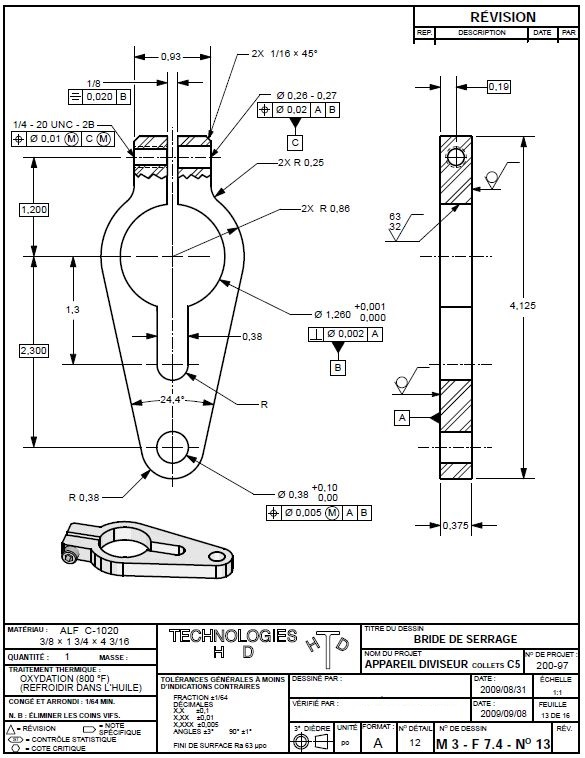
\includegraphics[scale=0.75]{dessin1.JPG}
\end{center}
\marginnote{0,25 pt}
\textcolor{red}{\textbf{MATIÈRE} : Acier 1020 : acier au carbone à faible trempabilité et à faible résistance à la traction qui a une valeur nominale de $0,22\%C$ et $0,55\%Mn$.} \\

\marginnote{0,25 pt}
\textcolor{red}{\textbf{QUANTITÉ} : Le dessin de définition nous indique que l'entreprise à seulement besoin d'une pièce.} \\
\marginnote{0,25 pt}
\textcolor{red}{\textbf{NORME} : Le dessin de définition nous indique que c'est la méthode du $3^{eme}$ dièdre qui est utilisée. La norme utilisé est la NF ISO 5456-2 et n'est pas la norme généralement utilisée en Europe. On remarque que le symbole utilisé est inversé par rapport à ce que nous avons appris en cours. Cela signifie par exemple que sur ce dessin, la vue de dessus est placée au-dessus de la vue de face.}


\newpage


\begin{exo} A partir de la pièce de la Figure du dessus, et d'après vos recherche, quel est le type de traitement utilisé sur la pièce, et quel est son intérêt ? \end{exo}

\marginnote{0,25 pt}
\textcolor{red}{\textbf{Type de traitement utilisé} : Thermique (et refroidissement)} \\


\marginnote{1 pt}
\textcolor{red}{\textbf{Intérêt du traitement} : Améliorer les caractéristiques des matériaux et rendre ceux-ci plus favorables à un emploi donné, à partir des modifications suivantes : Augmentation de la résistance à la rupture et de la limité élastique Rem, Re,
A \% en donnant une meilleure tenue de l'élément ; augmentation de la dureté, permettant à des pièces de mieux résister à l'usure ou aux chocs.}

\section{Quelles sont les différentes opérations d'usinage}
\subsection{Génération de surfaces}


\begin{exo} Quelle est la génératrice qui engendre un \textbf{cylindre} ? Quel est l'\textbf{axe de rotation} pour l'engendrer ? Vous ferez un schéma pour expliquez votre solution.\end{exo}

\textcolor{red}{\textbf{RÉPONSE} : Un cylindre sera généré par rotation d'un rectangle. L'axe de rotation pour l'engendrer peut être n'importe quel coté du rectangle.} \\

\marginnote{0,25 + 0,75 = 1 pt}
\textcolor{red}{\textbf{SCHÉMA} :}

%%%%%%%%%%%%%%%%%%%%%%%%%%%%%%%%%%%%%%%%%%%%%%%%%%%%%%%%%%%%%%%%%%%%%


\tikzset{every picture/.style={line width=0.75pt}} %set default line width to 0.75pt        

\begin{tikzpicture}[x=0.75pt,y=0.75pt,yscale=-1,xscale=1]
%uncomment if require: \path (0,234); %set diagram left start at 0, and has height of 234

%Shape: Rectangle [id:dp053180185031038496] 
\draw   (280,69) -- (334.5,69) -- (334.5,148) -- (280,148) -- cycle ;
%Shape: Circle [id:dp8654925518011107] 
\draw  [fill={rgb, 255:red, 0; green, 0; blue, 0 }  ,fill opacity=1 ] (276.25,69) .. controls (276.25,66.93) and (277.93,65.25) .. (280,65.25) .. controls (282.07,65.25) and (283.75,66.93) .. (283.75,69) .. controls (283.75,71.07) and (282.07,72.75) .. (280,72.75) .. controls (277.93,72.75) and (276.25,71.07) .. (276.25,69) -- cycle ;
%Shape: Circle [id:dp5864777646945023] 
\draw  [fill={rgb, 255:red, 0; green, 0; blue, 0 }  ,fill opacity=1 ] (330.75,69) .. controls (330.75,66.93) and (332.43,65.25) .. (334.5,65.25) .. controls (336.57,65.25) and (338.25,66.93) .. (338.25,69) .. controls (338.25,71.07) and (336.57,72.75) .. (334.5,72.75) .. controls (332.43,72.75) and (330.75,71.07) .. (330.75,69) -- cycle ;
%Shape: Circle [id:dp7492769468964013] 
\draw  [fill={rgb, 255:red, 0; green, 0; blue, 0 }  ,fill opacity=1 ] (276.25,148) .. controls (276.25,145.93) and (277.93,144.25) .. (280,144.25) .. controls (282.07,144.25) and (283.75,145.93) .. (283.75,148) .. controls (283.75,150.07) and (282.07,151.75) .. (280,151.75) .. controls (277.93,151.75) and (276.25,150.07) .. (276.25,148) -- cycle ;
%Shape: Circle [id:dp44435835510055854] 
\draw  [fill={rgb, 255:red, 0; green, 0; blue, 0 }  ,fill opacity=1 ] (330.75,148) .. controls (330.75,145.93) and (332.43,144.25) .. (334.5,144.25) .. controls (336.57,144.25) and (338.25,145.93) .. (338.25,148) .. controls (338.25,150.07) and (336.57,151.75) .. (334.5,151.75) .. controls (332.43,151.75) and (330.75,150.07) .. (330.75,148) -- cycle ;
%Straight Lines [id:da4218126727456757] 
\draw  [dash pattern={on 4.5pt off 4.5pt}]  (280.5,16) -- (279.5,200) ;
%Shape: Arc [id:dp3025341345021746] 
\draw  [draw opacity=0][dash pattern={on 0.84pt off 2.51pt}] (334.5,72.88) .. controls (334.5,89.37) and (309.88,102.75) .. (279.5,102.75) .. controls (249.12,102.75) and (224.5,89.37) .. (224.5,72.88) -- (279.5,72.88) -- cycle ; \draw  [dash pattern={on 0.84pt off 2.51pt}] (334.5,72.88) .. controls (334.5,89.37) and (309.88,102.75) .. (279.5,102.75) .. controls (249.12,102.75) and (224.5,89.37) .. (224.5,72.88) ;  
%Shape: Arc [id:dp8857131670993674] 
\draw  [draw opacity=0][dash pattern={on 0.84pt off 2.51pt}] (335,147.75) .. controls (335,147.75) and (335,147.75) .. (335,147.75) .. controls (335,147.75) and (335,147.75) .. (335,147.75) .. controls (335,164.25) and (310.38,177.63) .. (280,177.63) .. controls (249.62,177.63) and (225,164.25) .. (225,147.75) -- (280,147.75) -- cycle ; \draw  [dash pattern={on 0.84pt off 2.51pt}] (335,147.75) .. controls (335,147.75) and (335,147.75) .. (335,147.75) .. controls (335,147.75) and (335,147.75) .. (335,147.75) .. controls (335,164.25) and (310.38,177.63) .. (280,177.63) .. controls (249.62,177.63) and (225,164.25) .. (225,147.75) ;  
%Shape: Rectangle [id:dp7899007587639444] 
\draw   (437,70) -- (491.5,70) -- (491.5,149) -- (437,149) -- cycle ;
%Shape: Circle [id:dp3667961491428209] 
\draw  [fill={rgb, 255:red, 0; green, 0; blue, 0 }  ,fill opacity=1 ] (433.25,70) .. controls (433.25,67.93) and (434.93,66.25) .. (437,66.25) .. controls (439.07,66.25) and (440.75,67.93) .. (440.75,70) .. controls (440.75,72.07) and (439.07,73.75) .. (437,73.75) .. controls (434.93,73.75) and (433.25,72.07) .. (433.25,70) -- cycle ;
%Shape: Circle [id:dp5176595539481372] 
\draw  [fill={rgb, 255:red, 0; green, 0; blue, 0 }  ,fill opacity=1 ] (487.75,70) .. controls (487.75,67.93) and (489.43,66.25) .. (491.5,66.25) .. controls (493.57,66.25) and (495.25,67.93) .. (495.25,70) .. controls (495.25,72.07) and (493.57,73.75) .. (491.5,73.75) .. controls (489.43,73.75) and (487.75,72.07) .. (487.75,70) -- cycle ;
%Shape: Circle [id:dp46250530286829283] 
\draw  [fill={rgb, 255:red, 0; green, 0; blue, 0 }  ,fill opacity=1 ] (433.25,149) .. controls (433.25,146.93) and (434.93,145.25) .. (437,145.25) .. controls (439.07,145.25) and (440.75,146.93) .. (440.75,149) .. controls (440.75,151.07) and (439.07,152.75) .. (437,152.75) .. controls (434.93,152.75) and (433.25,151.07) .. (433.25,149) -- cycle ;
%Shape: Circle [id:dp34915097593765587] 
\draw  [fill={rgb, 255:red, 0; green, 0; blue, 0 }  ,fill opacity=1 ] (487.75,149) .. controls (487.75,146.93) and (489.43,145.25) .. (491.5,145.25) .. controls (493.57,145.25) and (495.25,146.93) .. (495.25,149) .. controls (495.25,151.07) and (493.57,152.75) .. (491.5,152.75) .. controls (489.43,152.75) and (487.75,151.07) .. (487.75,149) -- cycle ;
%Straight Lines [id:da3857421044824818] 
\draw  [dash pattern={on 4.5pt off 4.5pt}]  (437.5,17) -- (436.5,201) ;
%Shape: Can [id:dp537203860933638] 
\draw   (491.5,76.5) -- (491.5,153.5) .. controls (491.5,167.58) and (465.98,179) .. (434.5,179) .. controls (403.02,179) and (377.5,167.58) .. (377.5,153.5) -- (377.5,76.5) .. controls (377.5,62.42) and (403.02,51) .. (434.5,51) .. controls (465.98,51) and (491.5,62.42) .. (491.5,76.5) .. controls (491.5,90.58) and (465.98,102) .. (434.5,102) .. controls (403.02,102) and (377.5,90.58) .. (377.5,76.5) ;
%Curve Lines [id:da3459620769693932] 
\draw    (311,33) .. controls (310.52,30.41) and (311.38,28.92) .. (313.59,28.51) .. controls (316.02,27.9) and (317,26.54) .. (316.52,24.43) .. controls (316.5,21.89) and (317.58,20.67) .. (319.77,20.78) .. controls (322.22,20.74) and (323.58,19.51) .. (323.85,17.09) .. controls (323.93,14.92) and (325.21,13.98) .. (327.69,14.28) .. controls (330.06,14.76) and (331.42,13.95) .. (331.76,11.85) .. controls (332.66,9.53) and (334.29,8.76) .. (336.66,9.53) .. controls (338.51,10.59) and (340,10.04) .. (341.13,7.88) .. controls (342.44,5.75) and (343.98,5.31) .. (345.75,6.58) .. controls (347.87,7.82) and (349.68,7.46) .. (351.17,5.51) .. controls (352.33,3.66) and (353.94,3.47) .. (356,4.92) .. controls (357.49,6.48) and (359.12,6.39) .. (360.88,4.65) .. controls (362.77,2.97) and (364.41,2.98) .. (365.8,4.68) .. controls (367.55,6.45) and (369.19,6.56) .. (370.72,5.01) .. controls (372.8,3.57) and (374.43,3.78) .. (375.61,5.63) .. controls (377.15,7.58) and (378.76,7.88) .. (380.44,6.52) .. controls (382.66,5.32) and (384.47,5.77) .. (385.86,7.86) .. controls (386.71,9.85) and (388.25,10.33) .. (390.49,9.3) .. controls (392.36,8.2) and (393.86,8.76) .. (394.97,10.99) .. controls (395.94,13.22) and (397.38,13.86) .. (399.28,12.91) .. controls (401.64,12.24) and (403.2,13.06) .. (403.97,15.38) .. controls (404.58,17.68) and (406.04,18.59) .. (408.35,18.12) .. controls (410.72,17.76) and (412.07,18.76) .. (412.4,21.12) .. controls (412.55,23.43) and (413.77,24.51) .. (416.06,24.36) .. controls (418.39,24.37) and (419.47,25.53) .. (419.3,27.84) -- (420.03,28.74) -- (424.33,35.41) ;
\draw [shift={(425.5,38)}, rotate = 248.2] [fill={rgb, 255:red, 0; green, 0; blue, 0 }  ][line width=0.08]  [draw opacity=0] (8.93,-4.29) -- (0,0) -- (8.93,4.29) -- cycle    ;
%Shape: Rectangle [id:dp5538683804474747] 
\draw   (16,87) -- (70.5,87) -- (70.5,166) -- (16,166) -- cycle ;
%Shape: Circle [id:dp2907922544166326] 
\draw  [fill={rgb, 255:red, 0; green, 0; blue, 0 }  ,fill opacity=1 ] (12.25,87) .. controls (12.25,84.93) and (13.93,83.25) .. (16,83.25) .. controls (18.07,83.25) and (19.75,84.93) .. (19.75,87) .. controls (19.75,89.07) and (18.07,90.75) .. (16,90.75) .. controls (13.93,90.75) and (12.25,89.07) .. (12.25,87) -- cycle ;
%Shape: Circle [id:dp5203767132698423] 
\draw  [fill={rgb, 255:red, 0; green, 0; blue, 0 }  ,fill opacity=1 ] (66.75,87) .. controls (66.75,84.93) and (68.43,83.25) .. (70.5,83.25) .. controls (72.57,83.25) and (74.25,84.93) .. (74.25,87) .. controls (74.25,89.07) and (72.57,90.75) .. (70.5,90.75) .. controls (68.43,90.75) and (66.75,89.07) .. (66.75,87) -- cycle ;
%Shape: Circle [id:dp8431091422977719] 
\draw  [fill={rgb, 255:red, 0; green, 0; blue, 0 }  ,fill opacity=1 ] (12.25,166) .. controls (12.25,163.93) and (13.93,162.25) .. (16,162.25) .. controls (18.07,162.25) and (19.75,163.93) .. (19.75,166) .. controls (19.75,168.07) and (18.07,169.75) .. (16,169.75) .. controls (13.93,169.75) and (12.25,168.07) .. (12.25,166) -- cycle ;
%Shape: Circle [id:dp0036569023776089615] 
\draw  [fill={rgb, 255:red, 0; green, 0; blue, 0 }  ,fill opacity=1 ] (66.75,166) .. controls (66.75,163.93) and (68.43,162.25) .. (70.5,162.25) .. controls (72.57,162.25) and (74.25,163.93) .. (74.25,166) .. controls (74.25,168.07) and (72.57,169.75) .. (70.5,169.75) .. controls (68.43,169.75) and (66.75,168.07) .. (66.75,166) -- cycle ;
%Shape: Circle [id:dp19466055116674053] 
\draw  [fill={rgb, 255:red, 0; green, 0; blue, 0 }  ,fill opacity=1 ] (159.5,88) .. controls (159.5,85.93) and (161.18,84.25) .. (163.25,84.25) .. controls (165.32,84.25) and (167,85.93) .. (167,88) .. controls (167,90.07) and (165.32,91.75) .. (163.25,91.75) .. controls (161.18,91.75) and (159.5,90.07) .. (159.5,88) -- cycle ;
%Shape: Circle [id:dp7282142477705551] 
\draw  [fill={rgb, 255:red, 0; green, 0; blue, 0 }  ,fill opacity=1 ] (159.5,167) .. controls (159.5,164.93) and (161.18,163.25) .. (163.25,163.25) .. controls (165.32,163.25) and (167,164.93) .. (167,167) .. controls (167,169.07) and (165.32,170.75) .. (163.25,170.75) .. controls (161.18,170.75) and (159.5,169.07) .. (159.5,167) -- cycle ;
%Straight Lines [id:da47571279643329767] 
\draw    (163.25,88) -- (163.25,167) ;
%Curve Lines [id:da44846760597499435] 
\draw    (84,211.2) .. controls (86.15,209.6) and (88.24,209.67) .. (90.29,211.4) .. controls (91.3,213.1) and (92.89,213.15) .. (95.06,211.54) .. controls (96.17,209.91) and (97.77,209.95) .. (99.86,211.67) .. controls (101.96,213.4) and (103.57,213.44) .. (104.69,211.8) .. controls (106.89,210.19) and (108.51,210.23) .. (109.55,211.92) .. controls (111.68,213.63) and (113.31,213.67) .. (114.44,212.03) .. controls (116.66,210.41) and (118.3,210.44) .. (119.37,212.13) .. controls (121.54,213.84) and (123.19,213.88) .. (124.32,212.23) .. controls (126.55,210.6) and (128.21,210.63) .. (129.29,212.32) .. controls (131.48,214.02) and (133.15,214.05) .. (134.29,212.4) .. controls (136.54,210.77) and (138.22,210.79) .. (139.31,212.48) .. controls (141.53,214.17) and (143.21,214.2) .. (144.36,212.55) .. controls (146.63,210.91) and (148.31,210.93) .. (149.42,212.61) .. controls (151.66,214.3) and (153.35,214.32) .. (154.5,212.67) .. controls (156.78,211.02) and (158.48,211.04) .. (159.6,212.72) .. controls (161.86,214.41) and (163.56,214.42) .. (164.71,212.76) .. controls (167,211.11) and (168.71,211.13) .. (169.84,212.81) .. controls (170.97,214.48) and (172.68,214.49) .. (174.98,212.84) .. controls (176.13,211.18) and (177.85,211.19) .. (180.13,212.87) .. controls (181.27,214.54) and (182.99,214.55) .. (185.29,212.9) .. controls (186.44,211.24) and (188.17,211.25) .. (190.46,212.92) .. controls (191.6,214.59) and (193.32,214.59) .. (195.63,212.94) .. controls (196.78,211.27) and (197.93,211.27) .. (199.08,212.94) .. controls (201.38,214.61) and (203.11,214.62) .. (204.26,212.95) .. controls (206.57,211.29) and (208.29,211.29) .. (209.44,212.96) .. controls (211.74,214.63) and (213.47,214.63) .. (214.62,212.96) .. controls (216.93,211.29) and (218.65,211.29) .. (219.8,212.96) .. controls (220.95,214.63) and (222.68,214.62) .. (224.98,212.95) .. controls (226.13,211.28) and (227.85,211.28) .. (230.16,212.94) .. controls (231.31,214.61) and (233.04,214.6) .. (235.33,212.93) .. controls (236.47,211.26) and (238.19,211.26) .. (240.49,212.92) .. controls (241.64,214.58) and (243.36,214.57) .. (245.64,212.9) .. controls (246.78,211.23) and (247.92,211.22) .. (249.07,212.88) .. controls (251.36,214.54) and (253.08,214.53) .. (254.21,212.86) .. controls (256.48,211.19) and (258.18,211.18) .. (259.33,212.84) .. controls (261.61,214.49) and (263.31,214.48) .. (264.44,212.81) .. controls (266.69,211.13) and (268.39,211.12) .. (269.53,212.78) .. controls (271.8,214.43) and (273.5,214.42) .. (274.61,212.75) .. controls (276.85,211.07) and (278.54,211.06) .. (279.67,212.72) .. controls (281.92,214.37) and (283.6,214.36) .. (284.71,212.69) .. controls (286.93,211) and (288.6,210.99) .. (289.72,212.65) .. controls (291.95,214.3) and (293.62,214.29) .. (294.72,212.62) .. controls (296.91,210.93) and (298.57,210.92) .. (299.68,212.58) .. controls (301.89,214.23) and (303.54,214.22) .. (304.63,212.54) .. controls (306.8,210.86) and (308.44,210.85) .. (309.54,212.5) .. controls (311.73,214.15) and (313.36,214.14) .. (314.43,212.47) .. controls (316.58,210.78) and (318.19,210.77) .. (319.28,212.43) .. controls (321.44,214.08) and (323.05,214.06) .. (324.1,212.39) .. controls (326.22,210.7) and (328.35,210.69) .. (330.48,212.34) .. controls (331.55,214) and (333.13,213.99) .. (335.22,212.3) .. controls (336.26,210.63) and (337.83,210.61) .. (339.93,212.26) .. controls (340.98,213.92) and (342.54,213.91) .. (344.59,212.23) .. controls (346.64,210.54) and (348.18,210.53) .. (349.22,212.19) .. controls (351.27,213.84) and (353.31,213.83) .. (355.32,212.15) .. controls (356.31,210.48) and (357.82,210.47) .. (359.84,212.12) .. controls (361.85,213.77) and (363.34,213.75) .. (364.32,212.08) .. controls (366.29,210.41) and (368.25,210.4) .. (370.22,212.05) .. controls (371.21,213.71) and (372.66,213.7) .. (374.59,212.02) .. controls (376.5,210.34) and (378.42,210.33) .. (380.34,211.99) .. controls (381.29,213.65) and (382.71,213.64) .. (384.58,211.97) .. controls (386.45,210.29) and (388.31,210.28) .. (390.16,211.94) .. controls (391.09,213.61) and (392.46,213.6) .. (394.28,211.93) .. controls (396.09,210.26) and (397.89,210.25) .. (399.69,211.91) -- (399.69,211.91) -- (407.59,211.9) ;
\draw [shift={(410.2,211.9)}, rotate = 180] [fill={rgb, 255:red, 0; green, 0; blue, 0 }  ][line width=0.08]  [draw opacity=0] (8.93,-4.29) -- (0,0) -- (8.93,4.29) -- cycle    ;

% Text Node
\draw (292,45) node [anchor=north west][inner sep=0.75pt]   [align=left] {A};
% Text Node
\draw (343,46) node [anchor=north west][inner sep=0.75pt]   [align=left] {B};
% Text Node
\draw (285.75,151) node [anchor=north west][inner sep=0.75pt]   [align=left] {C};
% Text Node
\draw (340.25,151) node [anchor=north west][inner sep=0.75pt]   [align=left] {D};
% Text Node
\draw (449,46) node [anchor=north west][inner sep=0.75pt]   [align=left] {A};
% Text Node
\draw (500,47) node [anchor=north west][inner sep=0.75pt]   [align=left] {B};
% Text Node
\draw (442.75,152) node [anchor=north west][inner sep=0.75pt]   [align=left] {C};
% Text Node
\draw (497.25,152) node [anchor=north west][inner sep=0.75pt]   [align=left] {D};
% Text Node
\draw (29,63) node [anchor=north west][inner sep=0.75pt]   [align=left] {A};
% Text Node
\draw (79,64) node [anchor=north west][inner sep=0.75pt]   [align=left] {B};
% Text Node
\draw (21.75,169) node [anchor=north west][inner sep=0.75pt]   [align=left] {C};
% Text Node
\draw (76.25,169) node [anchor=north west][inner sep=0.75pt]   [align=left] {D};
% Text Node
\draw (175.25,64) node [anchor=north west][inner sep=0.75pt]   [align=left] {A};
% Text Node
\draw (169,170) node [anchor=north west][inner sep=0.75pt]   [align=left] {C};
% Text Node
\draw (19,9) node [anchor=north west][inner sep=0.75pt]  [font=\footnotesize] [align=left] {\begin{minipage}[lt]{42.19pt}\setlength\topsep{0pt}
Rectangle \\
générateur

\end{minipage}};
% Text Node
\draw (127,43) node [anchor=north west][inner sep=0.75pt]  [font=\footnotesize] [align=left] {Axe de rotation};
% Text Node
\draw (19.2,203.2) node [anchor=north west][inner sep=0.75pt]   [align=left] {Triangle};
% Text Node
\draw (418.4,203.2) node [anchor=north west][inner sep=0.75pt]   [align=left] {Cône};


\end{tikzpicture}
%%%%%%%%%%%%%%%%%%%%%%%%%%%%%%%%%%%%%%%%%%%%%%%%%%%%%%%%%%%%%%%%%%%%%%






\newpage


\begin{exo} Quelle est la génératrice qui engendre un \textbf{cône} ? Quel est l'\textbf{axe de rotation} pour l'engendrer ? Vous ferez un schéma pour expliquez votre solution.\end{exo}


\textcolor{red}{\textbf{RÉPONSE} : Un cône sera généré par rotation d'un triangle rectangle. L'axe de rotation pour l'engendrer doit être un des deux côté qui "touche" l'angle droit du triangle.} \\

\marginnote{0,25 + 0,75 = 1 pt}
\textcolor{red}{\textbf{SCHÉMA} :}

%%%%%%%%%%%%%%%%%%%%%%%%%%%%%%%%%%%%%%%%%%%%%%%%%%%%%%%%%%%%%%%%%%%%%%%%%%%%%%%%%


\tikzset{every picture/.style={line width=0.75pt}} %set default line width to 0.75pt        

\begin{tikzpicture}[x=0.75pt,y=0.75pt,yscale=-1,xscale=1]
%uncomment if require: \path (0,271); %set diagram left start at 0, and has height of 271

%Shape: Triangle [id:dp8224635078541052] 
\draw   (40,92) -- (120.5,201) -- (40,201) -- cycle ;
%Shape: Circle [id:dp08797442509248987] 
\draw  [fill={rgb, 255:red, 0; green, 0; blue, 0 }  ,fill opacity=1 ] (36.25,92) .. controls (36.25,89.93) and (37.93,88.25) .. (40,88.25) .. controls (42.07,88.25) and (43.75,89.93) .. (43.75,92) .. controls (43.75,94.07) and (42.07,95.75) .. (40,95.75) .. controls (37.93,95.75) and (36.25,94.07) .. (36.25,92) -- cycle ;
%Shape: Circle [id:dp3612015835968285] 
\draw  [fill={rgb, 255:red, 0; green, 0; blue, 0 }  ,fill opacity=1 ] (36.25,201) .. controls (36.25,198.93) and (37.93,197.25) .. (40,197.25) .. controls (42.07,197.25) and (43.75,198.93) .. (43.75,201) .. controls (43.75,203.07) and (42.07,204.75) .. (40,204.75) .. controls (37.93,204.75) and (36.25,203.07) .. (36.25,201) -- cycle ;
%Shape: Circle [id:dp5170669803791414] 
\draw  [fill={rgb, 255:red, 0; green, 0; blue, 0 }  ,fill opacity=1 ] (116.75,201) .. controls (116.75,198.93) and (118.43,197.25) .. (120.5,197.25) .. controls (122.57,197.25) and (124.25,198.93) .. (124.25,201) .. controls (124.25,203.07) and (122.57,204.75) .. (120.5,204.75) .. controls (118.43,204.75) and (116.75,203.07) .. (116.75,201) -- cycle ;
%Shape: Circle [id:dp5734599023477054] 
\draw  [fill={rgb, 255:red, 0; green, 0; blue, 0 }  ,fill opacity=1 ] (193.5,105) .. controls (193.5,102.93) and (195.18,101.25) .. (197.25,101.25) .. controls (199.32,101.25) and (201,102.93) .. (201,105) .. controls (201,107.07) and (199.32,108.75) .. (197.25,108.75) .. controls (195.18,108.75) and (193.5,107.07) .. (193.5,105) -- cycle ;
%Shape: Circle [id:dp1874186309492969] 
\draw  [fill={rgb, 255:red, 0; green, 0; blue, 0 }  ,fill opacity=1 ] (193.5,184) .. controls (193.5,181.93) and (195.18,180.25) .. (197.25,180.25) .. controls (199.32,180.25) and (201,181.93) .. (201,184) .. controls (201,186.07) and (199.32,187.75) .. (197.25,187.75) .. controls (195.18,187.75) and (193.5,186.07) .. (193.5,184) -- cycle ;
%Straight Lines [id:da0018975424044040956] 
\draw    (197.25,105) -- (197.25,184) ;
%Shape: Right Angle [id:dp8759584182398086] 
\draw  [color={rgb, 255:red, 208; green, 2; blue, 27 }  ,draw opacity=1 ][line width=2.25]  (40,190) -- (51,190) -- (51,201) ;
%Shape: Right Angle [id:dp4729839468260477] 
\draw  [color={rgb, 255:red, 208; green, 2; blue, 27 }  ,draw opacity=1 ][line width=2.25]  (197.25,176.75) -- (208.25,176.75) -- (208.25,187.75) ;
%Shape: Triangle [id:dp9879815646738546] 
\draw   (345,78) -- (425.5,187) -- (345,187) -- cycle ;
%Shape: Circle [id:dp9617806661779003] 
\draw  [fill={rgb, 255:red, 0; green, 0; blue, 0 }  ,fill opacity=1 ] (341.25,78) .. controls (341.25,75.93) and (342.93,74.25) .. (345,74.25) .. controls (347.07,74.25) and (348.75,75.93) .. (348.75,78) .. controls (348.75,80.07) and (347.07,81.75) .. (345,81.75) .. controls (342.93,81.75) and (341.25,80.07) .. (341.25,78) -- cycle ;
%Shape: Circle [id:dp7609271742822381] 
\draw  [fill={rgb, 255:red, 0; green, 0; blue, 0 }  ,fill opacity=1 ] (341.25,187) .. controls (341.25,184.93) and (342.93,183.25) .. (345,183.25) .. controls (347.07,183.25) and (348.75,184.93) .. (348.75,187) .. controls (348.75,189.07) and (347.07,190.75) .. (345,190.75) .. controls (342.93,190.75) and (341.25,189.07) .. (341.25,187) -- cycle ;
%Shape: Circle [id:dp38661710452665354] 
\draw  [fill={rgb, 255:red, 0; green, 0; blue, 0 }  ,fill opacity=1 ] (421.75,187) .. controls (421.75,184.93) and (423.43,183.25) .. (425.5,183.25) .. controls (427.57,183.25) and (429.25,184.93) .. (429.25,187) .. controls (429.25,189.07) and (427.57,190.75) .. (425.5,190.75) .. controls (423.43,190.75) and (421.75,189.07) .. (421.75,187) -- cycle ;
%Shape: Right Angle [id:dp25303517326381786] 
\draw  [color={rgb, 255:red, 208; green, 2; blue, 27 }  ,draw opacity=1 ][line width=2.25]  (345,176) -- (356,176) -- (356,187) ;
%Shape: Arc [id:dp04445146933373967] 
\draw  [draw opacity=0][dash pattern={on 0.84pt off 2.51pt}] (425.5,182.06) .. controls (425.5,182.06) and (425.5,182.06) .. (425.5,182.06) .. controls (425.5,199.22) and (389.68,213.13) .. (345.5,213.13) .. controls (301.32,213.13) and (265.5,199.22) .. (265.5,182.06) -- (345.5,182.06) -- cycle ; \draw  [dash pattern={on 0.84pt off 2.51pt}] (425.5,182.06) .. controls (425.5,182.06) and (425.5,182.06) .. (425.5,182.06) .. controls (425.5,199.22) and (389.68,213.13) .. (345.5,213.13) .. controls (301.32,213.13) and (265.5,199.22) .. (265.5,182.06) ;  
%Shape: Arc [id:dp1782033086904704] 
\draw  [draw opacity=0][dash pattern={on 0.84pt off 2.51pt}] (394.5,144.66) .. controls (394.5,144.66) and (394.5,144.66) .. (394.5,144.66) .. controls (394.5,144.66) and (394.5,144.66) .. (394.5,144.66) .. controls (394.5,155.51) and (372.56,164.31) .. (345.5,164.31) .. controls (318.44,164.31) and (296.5,155.51) .. (296.5,144.66) -- (345.5,144.66) -- cycle ; \draw  [dash pattern={on 0.84pt off 2.51pt}] (394.5,144.66) .. controls (394.5,144.66) and (394.5,144.66) .. (394.5,144.66) .. controls (394.5,144.66) and (394.5,144.66) .. (394.5,144.66) .. controls (394.5,155.51) and (372.56,164.31) .. (345.5,164.31) .. controls (318.44,164.31) and (296.5,155.51) .. (296.5,144.66) ;  
%Shape: Arc [id:dp45472268168527186] 
\draw  [draw opacity=0][dash pattern={on 0.84pt off 2.51pt}] (369.75,112.28) .. controls (369.75,112.28) and (369.75,112.28) .. (369.75,112.28) .. controls (369.75,121.14) and (358.67,128.31) .. (345,128.31) .. controls (331.33,128.31) and (320.25,121.14) .. (320.25,112.28) -- (345,112.28) -- cycle ; \draw  [dash pattern={on 0.84pt off 2.51pt}] (369.75,112.28) .. controls (369.75,112.28) and (369.75,112.28) .. (369.75,112.28) .. controls (369.75,121.14) and (358.67,128.31) .. (345,128.31) .. controls (331.33,128.31) and (320.25,121.14) .. (320.25,112.28) ;  
%Straight Lines [id:da6722424834663996] 
\draw  [dash pattern={on 4.5pt off 4.5pt}]  (344.5,10.75) -- (344.5,255.25) ;
%Shape: Triangle [id:dp11929842175482075] 
\draw   (549,78.5) -- (629.5,187.5) -- (549,187.5) -- cycle ;
%Shape: Circle [id:dp27570885327990746] 
\draw  [fill={rgb, 255:red, 0; green, 0; blue, 0 }  ,fill opacity=1 ] (545.25,78.5) .. controls (545.25,76.43) and (546.93,74.75) .. (549,74.75) .. controls (551.07,74.75) and (552.75,76.43) .. (552.75,78.5) .. controls (552.75,80.57) and (551.07,82.25) .. (549,82.25) .. controls (546.93,82.25) and (545.25,80.57) .. (545.25,78.5) -- cycle ;
%Shape: Circle [id:dp9465560514070064] 
\draw  [fill={rgb, 255:red, 0; green, 0; blue, 0 }  ,fill opacity=1 ] (545.25,187.5) .. controls (545.25,185.43) and (546.93,183.75) .. (549,183.75) .. controls (551.07,183.75) and (552.75,185.43) .. (552.75,187.5) .. controls (552.75,189.57) and (551.07,191.25) .. (549,191.25) .. controls (546.93,191.25) and (545.25,189.57) .. (545.25,187.5) -- cycle ;
%Shape: Circle [id:dp8921770232851238] 
\draw  [fill={rgb, 255:red, 0; green, 0; blue, 0 }  ,fill opacity=1 ] (625.75,187.5) .. controls (625.75,185.43) and (627.43,183.75) .. (629.5,183.75) .. controls (631.57,183.75) and (633.25,185.43) .. (633.25,187.5) .. controls (633.25,189.57) and (631.57,191.25) .. (629.5,191.25) .. controls (627.43,191.25) and (625.75,189.57) .. (625.75,187.5) -- cycle ;
%Shape: Right Angle [id:dp009923348549967903] 
\draw  [color={rgb, 255:red, 208; green, 2; blue, 27 }  ,draw opacity=1 ][line width=2.25]  (549,176.5) -- (560,176.5) -- (560,187.5) ;
%Shape: Arc [id:dp2704083490369322] 
\draw  [draw opacity=0] (629.5,184.56) .. controls (629.5,184.56) and (629.5,184.56) .. (629.5,184.56) .. controls (629.5,201.72) and (593.68,215.63) .. (549.5,215.63) .. controls (505.32,215.63) and (469.5,201.72) .. (469.5,184.56) -- (549.5,184.56) -- cycle ; \draw   (629.5,184.56) .. controls (629.5,184.56) and (629.5,184.56) .. (629.5,184.56) .. controls (629.5,201.72) and (593.68,215.63) .. (549.5,215.63) .. controls (505.32,215.63) and (469.5,201.72) .. (469.5,184.56) ;  
%Shape: Arc [id:dp2516357935241633] 
\draw  [draw opacity=0][dash pattern={on 0.84pt off 2.51pt}] (598.5,145.16) .. controls (598.5,145.16) and (598.5,145.16) .. (598.5,145.16) .. controls (598.5,145.16) and (598.5,145.16) .. (598.5,145.16) .. controls (598.5,156.01) and (576.56,164.81) .. (549.5,164.81) .. controls (522.44,164.81) and (500.5,156.01) .. (500.5,145.16) -- (549.5,145.16) -- cycle ; \draw  [dash pattern={on 0.84pt off 2.51pt}] (598.5,145.16) .. controls (598.5,145.16) and (598.5,145.16) .. (598.5,145.16) .. controls (598.5,145.16) and (598.5,145.16) .. (598.5,145.16) .. controls (598.5,156.01) and (576.56,164.81) .. (549.5,164.81) .. controls (522.44,164.81) and (500.5,156.01) .. (500.5,145.16) ;  
%Straight Lines [id:da26129869552810847] 
\draw    (549,78.5) -- (469.5,184.56) ;
%Curve Lines [id:da191685767612658] 
\draw    (380.33,57.67) .. controls (379.89,55.05) and (380.79,53.55) .. (383.02,53.16) .. controls (385.49,52.63) and (386.56,51.28) .. (386.22,49.12) .. controls (386.05,46.87) and (387.28,45.67) .. (389.89,45.51) .. controls (392.06,45.88) and (393.22,44.96) .. (393.38,42.76) .. controls (394.16,40.24) and (395.64,39.3) .. (397.83,39.94) .. controls (399.94,40.7) and (401.54,39.89) .. (402.65,37.52) .. controls (403.47,35.36) and (404.93,34.77) .. (407.04,35.76) .. controls (409.07,36.83) and (410.6,36.33) .. (411.64,34.28) .. controls (412.82,32.23) and (414.42,31.83) .. (416.45,33.06) .. controls (418.4,34.36) and (420.06,34.05) .. (421.42,32.12) .. controls (422.89,30.21) and (424.6,29.98) .. (426.54,31.42) .. controls (428.42,32.91) and (430.17,32.76) .. (431.79,30.97) .. controls (433.5,29.22) and (434.98,29.15) .. (436.23,30.78) .. controls (438.04,32.43) and (439.84,32.42) .. (441.64,30.77) .. controls (443.52,29.15) and (445.04,29.2) .. (446.19,30.92) .. controls (447.9,32.69) and (449.74,32.82) .. (451.69,31.31) .. controls (453.7,29.83) and (455.23,29.99) .. (456.28,31.79) .. controls (457.89,33.68) and (459.72,33.93) .. (461.78,32.55) .. controls (463.27,31.1) and (464.79,31.36) .. (466.34,33.33) .. controls (467.82,35.32) and (469.33,35.62) .. (470.87,34.24) .. controls (473.04,33.03) and (474.83,33.45) .. (476.24,35.5) .. controls (477.57,37.57) and (479.03,37.97) .. (480.64,36.68) .. controls (482.86,35.59) and (484.59,36.11) .. (485.82,38.24) .. controls (486.97,40.38) and (488.65,40.96) .. (490.86,39.97) .. controls (492.55,38.81) and (493.91,39.33) .. (494.95,41.52) .. controls (495.9,43.71) and (497.47,44.37) .. (499.68,43.5) .. controls (501.91,42.69) and (503.42,43.39) .. (504.21,45.62) .. controls (504.89,47.84) and (506.32,48.59) .. (508.51,47.87) .. controls (510.72,47.2) and (512.29,48.12) .. (513.21,50.63) .. controls (513.56,52.84) and (514.8,53.67) .. (516.94,53.12) .. controls (519.51,52.95) and (520.83,53.96) .. (520.91,56.15) -- (521.96,57.04) -- (527.47,62.56) ;
\draw [shift={(529,64.5)}, rotate = 233.7] [fill={rgb, 255:red, 0; green, 0; blue, 0 }  ][line width=0.08]  [draw opacity=0] (8.93,-4.29) -- (0,0) -- (8.93,4.29) -- cycle    ;
%Curve Lines [id:da6139465820801802] 
\draw    (118.4,237.6) .. controls (120.56,236) and (122.69,236.07) .. (124.78,237.8) .. controls (125.82,239.5) and (127.47,239.55) .. (129.73,237.95) .. controls (130.89,236.31) and (132.58,236.35) .. (134.8,238.08) .. controls (135.91,239.78) and (137.64,239.82) .. (140,238.21) .. controls (141.21,236.58) and (142.39,236.61) .. (143.53,238.3) .. controls (145.88,240.02) and (147.68,240.06) .. (148.93,238.42) .. controls (151.4,236.81) and (153.24,236.84) .. (154.44,238.53) .. controls (155.65,240.22) and (157.52,240.26) .. (160.06,238.64) .. controls (161.35,237) and (162.62,237.02) .. (163.86,238.71) .. controls (166.4,240.42) and (168.33,240.46) .. (169.65,238.81) .. controls (170.98,237.16) and (172.28,237.19) .. (173.56,238.88) .. controls (176.17,240.59) and (178.16,240.62) .. (179.51,238.97) .. controls (180.87,237.32) and (182.21,237.33) .. (183.52,239.02) .. controls (186.2,240.73) and (188.23,240.76) .. (189.61,239.11) .. controls (191,237.46) and (192.37,237.47) .. (193.72,239.16) .. controls (196.46,240.86) and (198.53,240.88) .. (199.94,239.23) .. controls (201.35,237.58) and (202.75,237.59) .. (204.13,239.28) .. controls (205.52,240.96) and (207.63,240.98) .. (210.48,239.34) .. controls (211.91,237.69) and (213.33,237.7) .. (214.74,239.38) .. controls (216.15,241.06) and (217.59,241.07) .. (219.04,239.42) .. controls (220.49,237.77) and (222.66,237.79) .. (225.53,239.48) .. controls (226.96,241.15) and (228.42,241.16) .. (229.89,239.51) .. controls (231.36,237.86) and (232.82,237.87) .. (234.27,239.54) .. controls (235.72,241.22) and (237.19,241.23) .. (238.67,239.58) .. controls (240.16,237.92) and (242.37,237.93) .. (245.31,239.62) .. controls (246.78,241.29) and (248.27,241.3) .. (249.77,239.64) .. controls (251.26,237.99) and (252.75,238) .. (254.24,239.67) .. controls (255.72,241.34) and (257.21,241.35) .. (258.72,239.69) .. controls (260.23,238.03) and (262.48,238.04) .. (265.48,239.72) .. controls (266.98,241.39) and (268.49,241.4) .. (270,239.74) .. controls (271.51,238.08) and (273.02,238.09) .. (274.53,239.76) .. controls (276.04,241.43) and (277.55,241.44) .. (279.07,239.77) .. controls (280.59,238.11) and (282.11,238.12) .. (283.62,239.79) .. controls (285.13,241.46) and (287.41,241.47) .. (290.45,239.81) .. controls (291.98,238.14) and (293.5,238.15) .. (295.02,239.82) .. controls (296.54,241.49) and (298.06,241.49) .. (299.59,239.83) .. controls (301.12,238.16) and (302.64,238.17) .. (304.16,239.84) .. controls (305.68,241.51) and (307.2,241.51) .. (308.73,239.84) .. controls (310.26,238.18) and (312.54,238.18) .. (315.59,239.85) .. controls (317.11,241.52) and (318.63,241.53) .. (320.16,239.86) .. controls (321.68,238.19) and (323.2,238.19) .. (324.72,239.86) .. controls (326.24,241.53) and (327.76,241.53) .. (329.28,239.86) .. controls (330.8,238.19) and (332.32,238.19) .. (333.84,239.86) .. controls (335.35,241.53) and (336.87,241.53) .. (338.38,239.86) .. controls (341.41,238.19) and (343.67,238.19) .. (345.18,239.86) .. controls (346.69,241.53) and (348.2,241.53) .. (349.71,239.86) .. controls (351.21,238.19) and (352.71,238.19) .. (354.22,239.86) .. controls (355.72,241.53) and (357.22,241.53) .. (358.71,239.86) .. controls (360.2,238.19) and (362.44,238.18) .. (365.43,239.85) .. controls (366.92,241.52) and (368.4,241.51) .. (369.88,239.84) .. controls (371.36,238.17) and (372.84,238.17) .. (374.32,239.84) .. controls (375.8,241.5) and (377.27,241.5) .. (378.74,239.83) .. controls (380.2,238.16) and (382.39,238.16) .. (385.32,239.82) .. controls (386.78,241.48) and (388.24,241.48) .. (389.69,239.81) .. controls (391.14,238.14) and (392.58,238.14) .. (394.03,239.8) .. controls (395.47,241.47) and (397.62,241.46) .. (400.48,239.79) .. controls (401.91,238.12) and (403.33,238.11) .. (404.76,239.78) .. controls (406.18,241.44) and (407.59,241.44) .. (409,239.77) .. controls (410.4,238.1) and (412.5,238.09) .. (415.31,239.75) .. controls (416.7,241.42) and (418.09,241.41) .. (419.47,239.74) .. controls (420.84,238.07) and (422.22,238.07) .. (423.6,239.73) .. controls (426.33,241.39) and (428.38,241.39) .. (429.73,239.72) .. controls (431.08,238.05) and (432.42,238.04) .. (433.77,239.7) .. controls (436.44,241.36) and (438.44,241.36) .. (439.76,239.69) .. controls (441.07,238.02) and (442.38,238.01) .. (443.7,239.68) .. controls (446.3,241.33) and (448.24,241.33) .. (449.53,239.66) .. controls (450.8,237.99) and (452.71,237.98) .. (455.26,239.64) .. controls (456.53,241.31) and (457.78,241.3) .. (459.03,239.63) .. controls (460.27,237.96) and (462.12,237.96) .. (464.59,239.61) .. controls (465.82,241.28) and (467.63,241.27) .. (470.04,239.6) .. controls (471.23,237.93) and (472.42,237.92) .. (473.61,239.59) .. controls (475.96,241.25) and (477.71,241.24) .. (478.86,239.57) .. controls (481.15,237.9) and (482.86,237.9) .. (483.99,239.56) .. controls (486.23,241.22) and (487.9,241.22) .. (489,239.55) .. controls (491.17,237.88) and (492.8,237.87) .. (493.87,239.54) .. controls (495.99,241.2) and (497.57,241.2) .. (498.61,239.53) .. controls (500.66,237.86) and (502.69,237.85) .. (504.7,239.52) .. controls (505.69,241.18) and (507.16,241.18) .. (509.1,239.51) -- (511.95,239.51) -- (518.77,239.5) ;
\draw [shift={(521.4,239.5)}, rotate = 180] [fill={rgb, 255:red, 0; green, 0; blue, 0 }  ][line width=0.08]  [draw opacity=0] (8.93,-4.29) -- (0,0) -- (8.93,4.29) -- cycle    ;

% Text Node
\draw (52,75) node [anchor=north west][inner sep=0.75pt]   [align=left] {A};
% Text Node
\draw (24.75,182) node [anchor=north west][inner sep=0.75pt]   [align=left] {B};
% Text Node
\draw (122.5,177.75) node [anchor=north west][inner sep=0.75pt]   [align=left] {C};
% Text Node
\draw (178.25,90) node [anchor=north west][inner sep=0.75pt]   [align=left] {A};
% Text Node
\draw (178,178) node [anchor=north west][inner sep=0.75pt]   [align=left] {B};
% Text Node
\draw (10,20) node [anchor=north west][inner sep=0.75pt]  [font=\footnotesize] [align=left] {\begin{minipage}[lt]{67.73pt}\setlength\topsep{0pt}
Triangle \\ rectangle \\ générateur
\end{minipage}};
% Text Node
\draw (160,33) node [anchor=north west][inner sep=0.75pt]  [font=\footnotesize] [align=left] {Axe de rotation :\\Un des deux côtés\\à "angle droit"};
% Text Node
\draw (357,61) node [anchor=north west][inner sep=0.75pt]   [align=left] {A};
% Text Node
\draw (329.75,168) node [anchor=north west][inner sep=0.75pt]   [align=left] {B};
% Text Node
\draw (427.5,163.75) node [anchor=north west][inner sep=0.75pt]   [align=left] {C};
% Text Node
\draw (561,61.5) node [anchor=north west][inner sep=0.75pt]   [align=left] {A};
% Text Node
\draw (533.75,168.5) node [anchor=north west][inner sep=0.75pt]   [align=left] {B};
% Text Node
\draw (631.5,164.25) node [anchor=north west][inner sep=0.75pt]   [align=left] {C};
% Text Node
\draw (53.6,229.6) node [anchor=north west][inner sep=0.75pt]   [align=left] {Triangle};
% Text Node
\draw (531.8,229.6) node [anchor=north west][inner sep=0.75pt]   [align=left] {Cône};


\end{tikzpicture}
%%%%%%%%%%%%%%%%%%%%%%%%%%%%%%%%%%%%%%%%%%%%%%%%%%%%%%%%%%%%%%%%%%%%%%%%%%%%%%



\newpage

\subsection{Le fraisage}
\begin{exo} Complétez le tableau d'opération d'usinage en tournage sur le document réponse. Vous devrez renseigner le ou les noms des opérations, la ou les formes/surfaces engendrées et enfin le ou les noms complets des outils.  \end{exo}
\marginnote{0,25 pt / réponse \\ = 3,75 pts}
\begin{center}
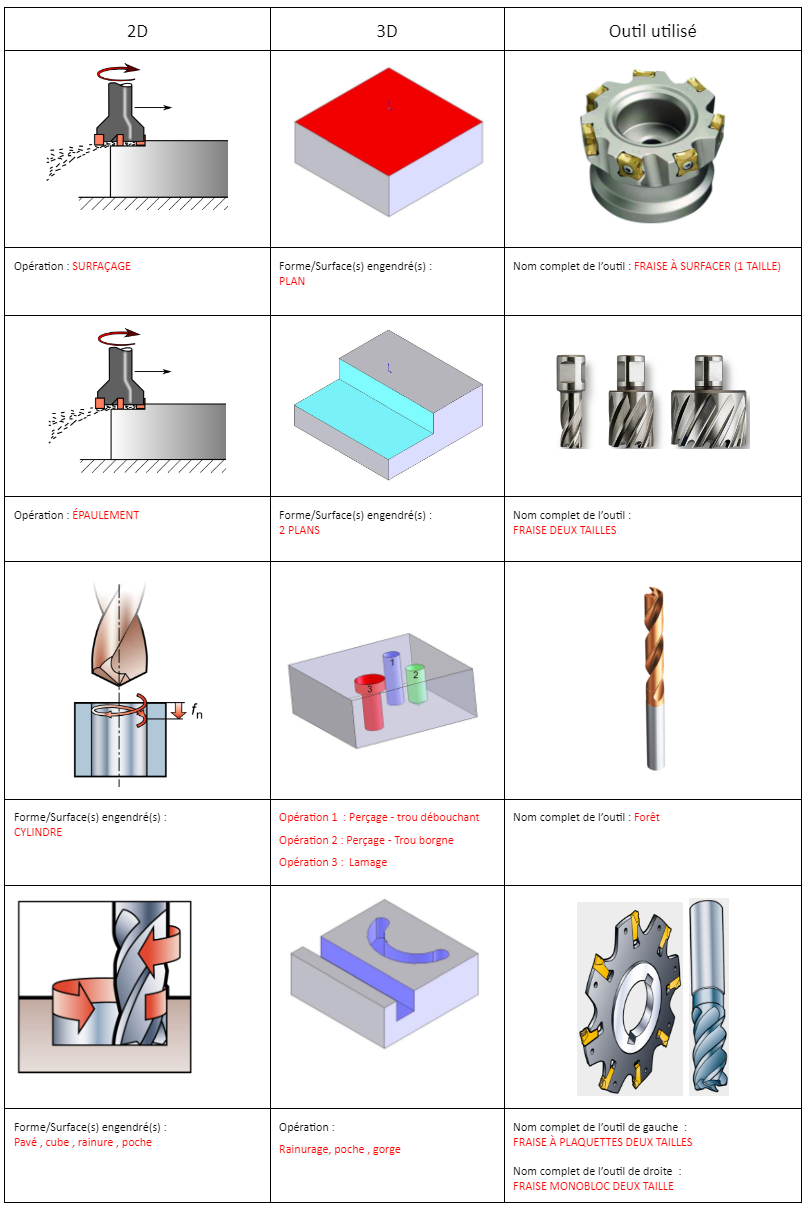
\includegraphics[scale=1.1]{CORR1.png}
\end{center}

\newpage

\subsection{Le tournage}
\begin{exo} Complétez le tableau d'opération d'usinage en fraisage sur le document réponse. Vous devrez renseigner le ou les noms des opérations, la ou les formes/surfaces engendrées et enfin le ou les noms complet des outils.  \end{exo}
\marginnote{0,25 pt / réponse \\ = 3,25 pts}
\begin{center}
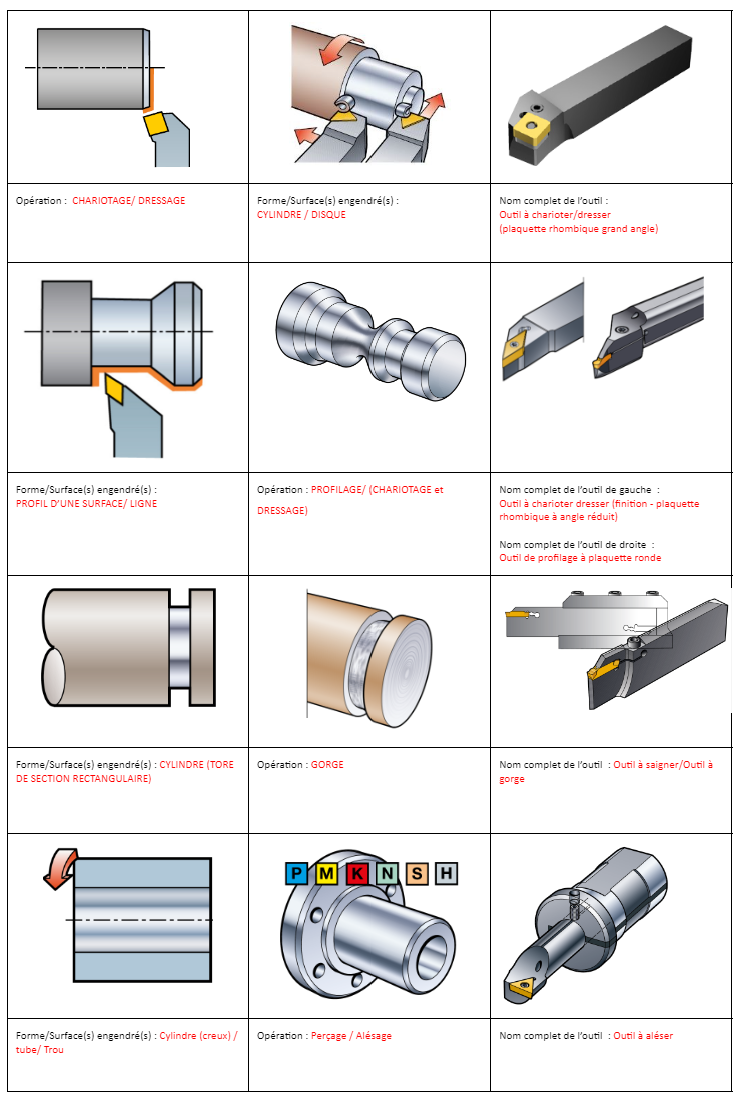
\includegraphics[scale=1.1]{CORR2.png}
\end{center}

\newpage

\section{Désignation des outils}
\subsection{Introduction}

\begin{exo} Quelles peuvent être les contraintes extérieures qui agissent sur le systèmes d'attache lors d'un usinage ? Vous citerez au moins 4 contraintes.\end{exo}
\marginnote{0,25 x 4 = 1 pt}
\begin{center}
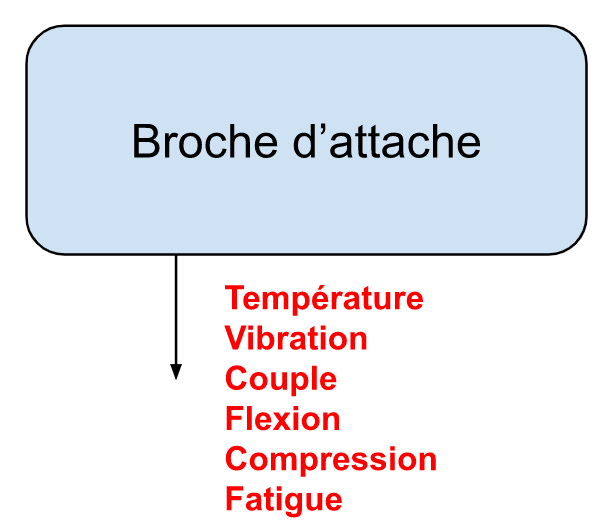
\includegraphics[scale=0.8]{CORR3.png}
\end{center}

\begin{exo} Quelles doivent être les caractéristiques principales des broches d'attaches ? Vous citerez au moins 3 caractéristiques.\end{exo}

\marginnote{0,25 x 3 = 0,75 pt}
\textcolor{red}{Pour réduire les temps morts, il faut que l'interface de broche autorise des changements rapides d'outils. Pendant l'usinage, il est essentiel que l'accouplement entre la broche et l'outil soit résistant et supporte sans problèmes les forces de coupe. Il est important d'avoir une interface avec une bonne résistance à la flexion et capable de transmettre le couple.}


\begin{enumerate}[1)]
    \item \textcolor{red}{\textbf{Résistance à la flexion} : La résistance à la flexion est particulièrement importante pour avoir un process de coupe stable avec des outils longs ou pour des coupes lourdes.}
    \item \textcolor{red}{\textbf{Transmission du couple} : Les opérations avec de grands diamètres sont les plus sensibles. La charge appliquée à distance de l'axe de la broche (Couple = Force x Rayon) doit être contrée par une surface d'entraînement plus importante.}
    \item \textcolor{red}{\textbf{Positionnement précis du centre de l'outil} : Pour la répétabilité et la sécurité de la production, surtout dans les opérations de tournage}
\end{enumerate}


\newpage

\begin{exo} A l’aide du graphique, \textbf{justifiez} quelle est l’attache avec la meilleure transmission du couple pour les essais effectués. \end{exo}

\begin{minipage}{.55\linewidth}
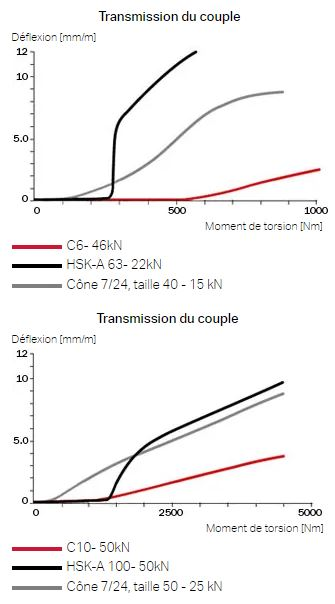
\includegraphics[scale=0.8]{T1.JPG}
\end{minipage}
\begin{minipage}{.44\linewidth}
\marginnote{1,25 pt}
\textcolor{red}{Les graphiques montrent que Coromant Capto C6 a une résistance au couple 2.29 fois plus élevée que HSK-A 63. L'angle de torsion est 7.1 fois meilleur. Pour C10, la résistance au couple est 1.85 fois meilleure et l'angle de torsion est 4 fois plus élevé que pour HSK-A 100. Pour les deux tests, c'est l'outil \underline{Coromant C} qui à les meilleures performances : la meilleure résistance à la déflexion.}
\end{minipage}


\newpage


\begin{exo} Conclure sur la pertinence d'avoir plusieurs technologie d'attache et forme différentes pour construire une liaison encastrement entre la machine et l'outil.
\end{exo}
\marginnote{1 pt}
\textcolor{red}{Au fur et à mesure de la recherche, plusieurs technologies d'attache ont été conçu, elles permettent de s'adapter aux différents besoins. Une attache avec une grande surface de contact sera privilégiée si le couple transmis est grand. A l'inverse, si le couple est plus faible, on pourra se diriger vers une attache moins performante sur la transmission du couple, ce qui nous fera économiser sur le montant unitaire des Porte-Outils.}


\subsection{Les outils en tournage}

\begin{exo} Nommer les différents  éléments de l’outil d’usinage à l'aide des mots
indiqués. \end{exo}
\marginnote{0,25 pt/réponse \\ = 1,5 pt}
\begin{minipage}{.55\linewidth}
\begin{itemize}
    \item Porte-outil;
    \item Sortie huile de coupe
    \item Liaison vis sans fin
\end{itemize} 
\end{minipage}
\begin{minipage}{.44\linewidth}
\begin{itemize}
    \item Plaquettes
    \item Cales
    \item Porte plaquette
\end{itemize} 
\end{minipage}
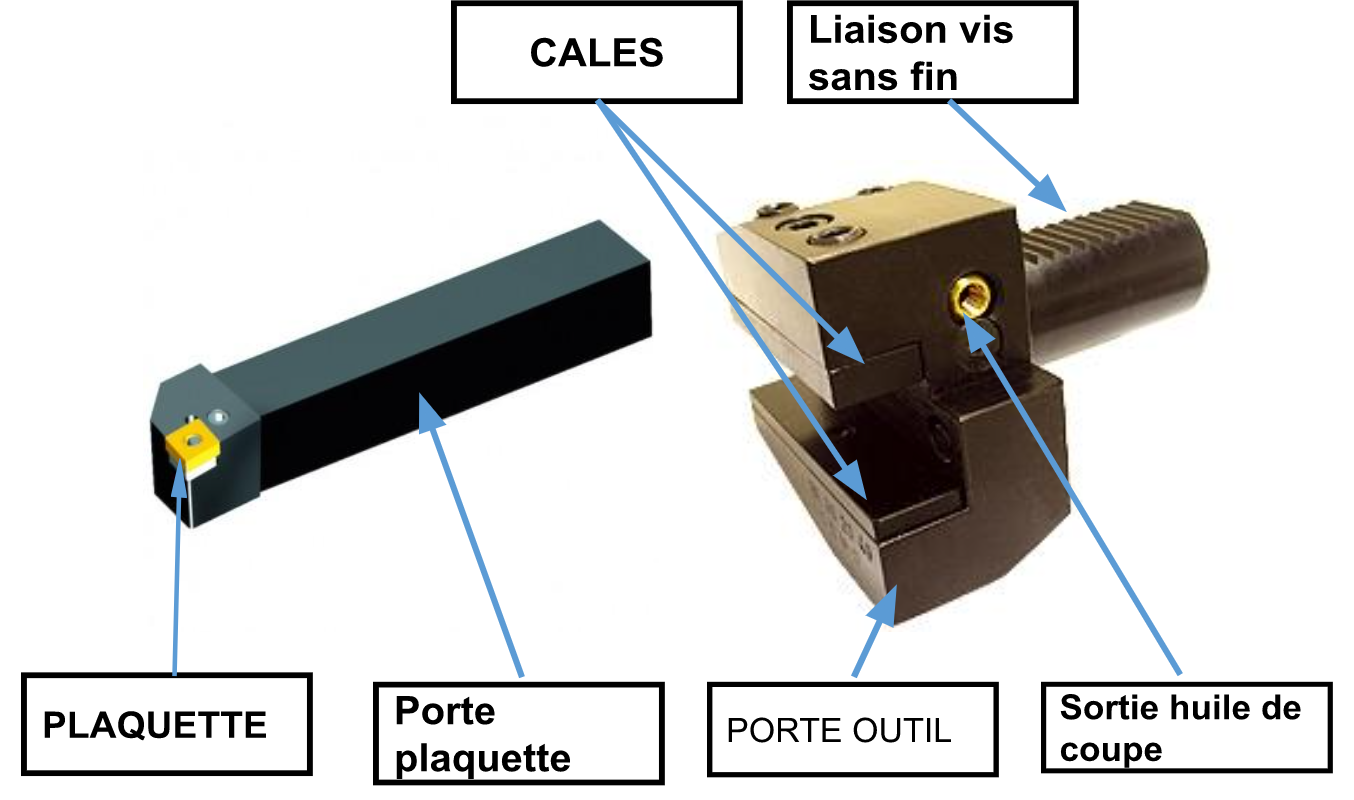
\includegraphics[scale=0.75]{CORR4.png}

\newpage

\subsection{Les outils en fraisage}

\begin{exo} Nommez les différents éléments de l’outil d’usinage figure à l'aide des mots
indiques dans le dossier réponse. \end{exo}
\marginnote{0,25 pt/réponse \\ = 1,5 pt}

\begin{minipage}{.55\linewidth}
\begin{itemize}
    \item  \textcolor{red}{4} Porte-outil ;
    \item  \textcolor{red}{6} Foret monobloc;
    \item \textcolor{red}{2} Clavette d'entraînement (transmission du couple);
\end{itemize} 
\end{minipage}
\begin{minipage}{.44\linewidth}
\begin{itemize}
    \item  \textcolor{red}{5} Outil;
    \item \textcolor{red}{3} Dispositif de serrage;
    \item  \textcolor{red}{1} Magasin outil / Tourelle;
\end{itemize} 
\end{minipage}


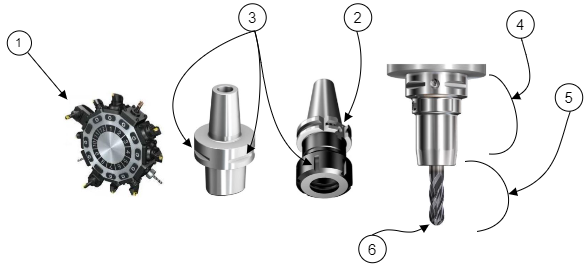
\includegraphics[scale=0.95]{FF1.png}




\section{Sélection des plaquettes - Application}
\subsection{Fabrication des plaquettes d'usinages}

\begin{exo} Quel est le type de procédé utilisé pour lier le mélange de poudre dans le processus de fabrication des plaquettes ?\end{exo}
\marginnote{0,5 pt}

\textcolor{red}{Procédé de PRESSAGE (voir poinçonnage). Réponse en plus : \\
Le pressage demande un ensemble d'outils : Poinçons supérieur et inférieur, Goujon central, Moule. Procédure de pressage : La poudre est versée dans le moule, Les poinçons se resserrent (20 à 50 tonnes), La plaquette est extraite et placée par un automate sur un support graphite, Un échantillonnage aléatoire est effectué pour vérifier le poids. A ce stade, les plaquettes sont poreuses à 50 \%.}


\begin{exo} Expliquez en quoi consiste un procédé de \textbf{frittage}.\end{exo}
\marginnote{2 pts}

\textcolor{red}{Il consiste à chauffer un corps contenant des matériaux différents, qui vont réagir ensemble grâce à leur nature chimique différentes.\\
Le frittage comporte les étapes suivantes : \\
- Les plateaux avec les plaquettes sont mis dans un four de frittage. \\
- La température est portée à ~1400°C . \\
- Le cobalt fond et agit comme liant. \\
- La taille des plaquettes réduit de 18 \% dans toutes les directions pendant le frittage, soit environ 50 \% en volume.}


\subsection{Partie active des outils coupant}

\begin{exo} Trouvez le noms des différents éléments de la figure du dessous qui constituent la zone de coupe des outils en vous aidant des mots indiqués.\end{exo}

\marginnote{0,25 pt x 14 \\ = 3,5 pt}
\begin{minipage}{.55\linewidth}
\begin{itemize}
    \item Arête de coupe \textcolor{red}{4, 7, 13} ;
    \item Face en dépouille \textcolor{red}{5, 14} ;
    \item Goujure \textcolor{red}{9} ;
    \item Face de coupe \textcolor{red}{2, 6} ;
\end{itemize} 
\end{minipage}
\begin{minipage}{.44\linewidth}
\begin{itemize}
    \item Bec de l'outil (rayon de bec) \textcolor{red}{3, 8, 12}  ;
    \item Angle d'hélice \textcolor{red}{10} ;
    \item Listel \textcolor{red}{11} ;
    \item Brise copeaux \textcolor{red}{1} ;
\end{itemize} 
\end{minipage}

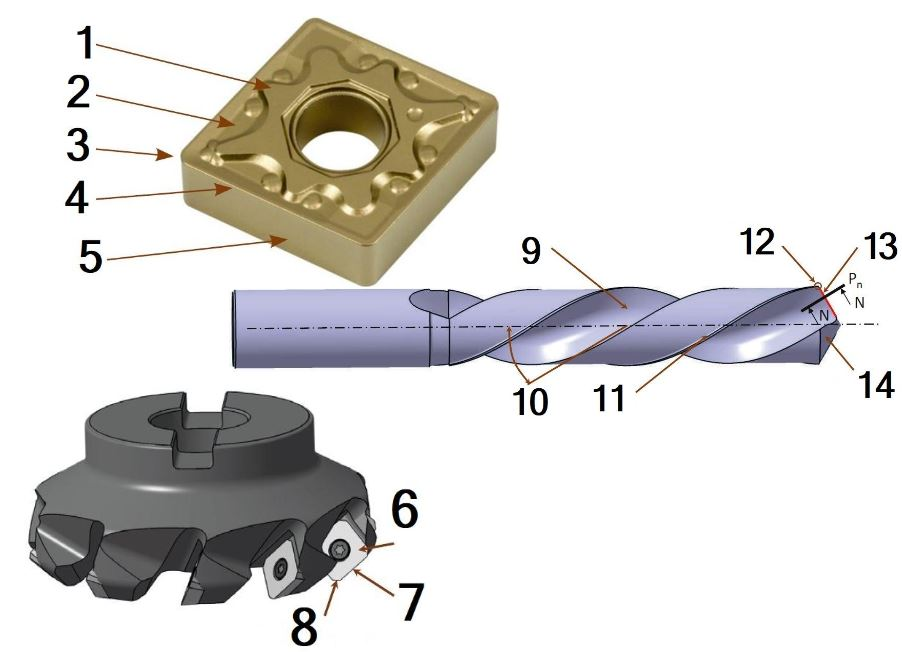
\includegraphics[scale=0.6]{PLA20.JPG}


\newpage

\begin{exo} En vous aidant de la figure ci-dessous comparez les plaquettes destinées à l'ébauche et à la finition. Comment les valeurs changent-elles de l'ébauche à la finition ?\end{exo}

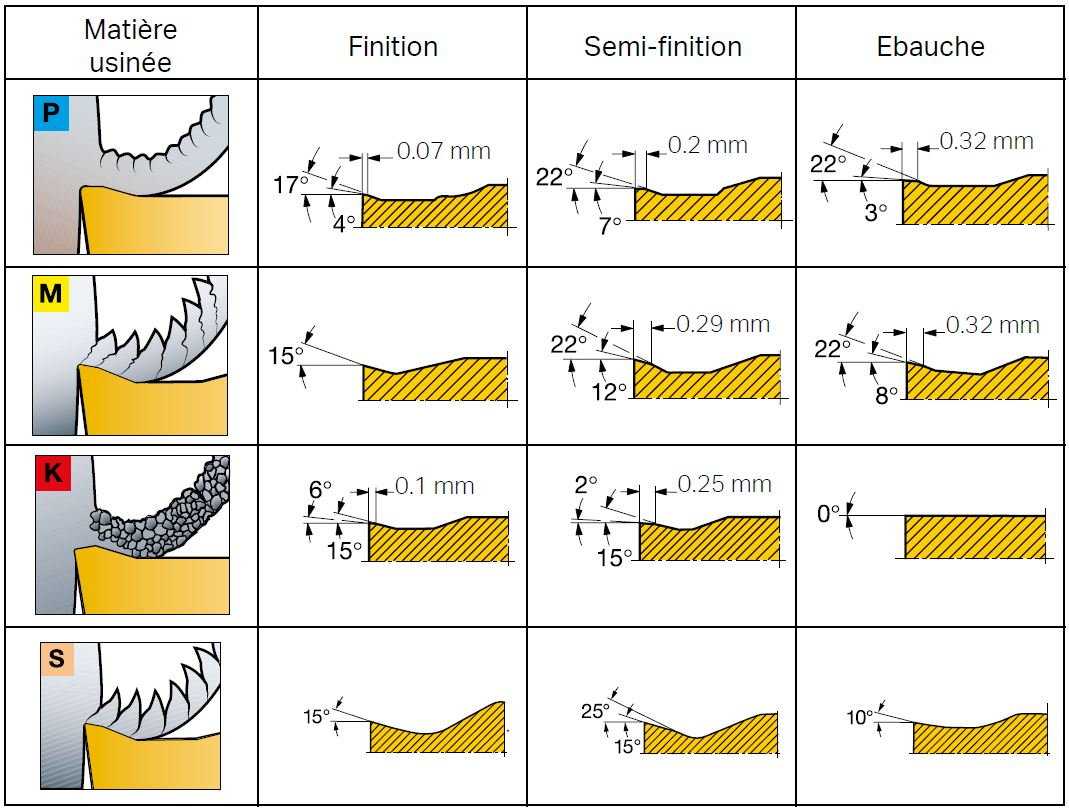
\includegraphics[scale=0.5]{PLA21.JPG}


\marginnote{1,5 pt}
\textcolor{red}{On remarque que les valeurs d'angle et de distances diminues de l'ébauche à la finition. En effet, on veut réduire les efforts de flexions, les vibrations et améliorer la précision et l'état de surface.\\
Le matériau usiner change les valeurs et on a parfois des angles plus grand en finition, mais on joue avec la valeurs des différents paramètre :\\
Angle de dépouille $\alpha$ : il a un impact sur le frottement entre l’outil et la pièce et par
conséquent il influe sur la durée de vie de l’outil \\
Angle de taillant $\beta$ : il a un impact sur la résistance à la rupture du taillant \\
Angle de coupe $\lambda$ : il a un impact sur les efforts de coupe, la puissance consommée, le flux de chaleur.}

\newpage


\begin{exo} Cherchez la signification des termes P, M, K, N, S, H présent sur la figure ci-dessous. \end{exo}
\marginnote{0,25 x 6 = 1,5 pt}
\begin{center}
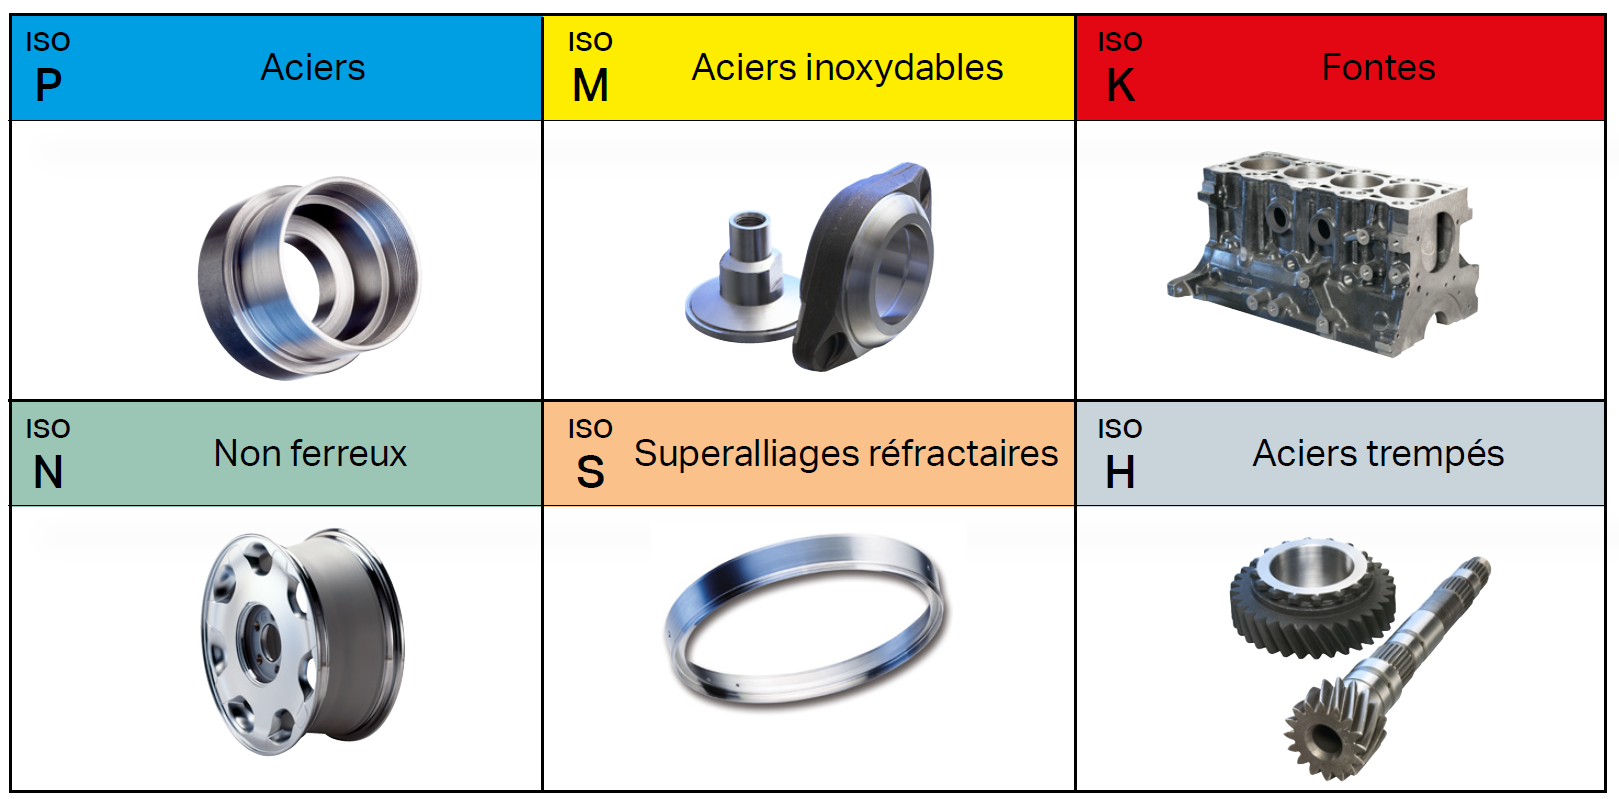
\includegraphics[width=0.8\linewidth]{CORR5.png}
\end{center}


\begin{exo} Ces informations concernent-elles l'outil ou la pièce ? \end{exo}

\marginnote{0,5 pt}


\textcolor{red}{Ces informations concernent la matière usinée, donc la pièce.}


\newpage


\begin{exo} Répartissez les plaquettes dans le bon ordre sur le graphe. \end{exo}
\marginnote{0,25 x 7 \\ = 1,75 pt}
\begin{center}
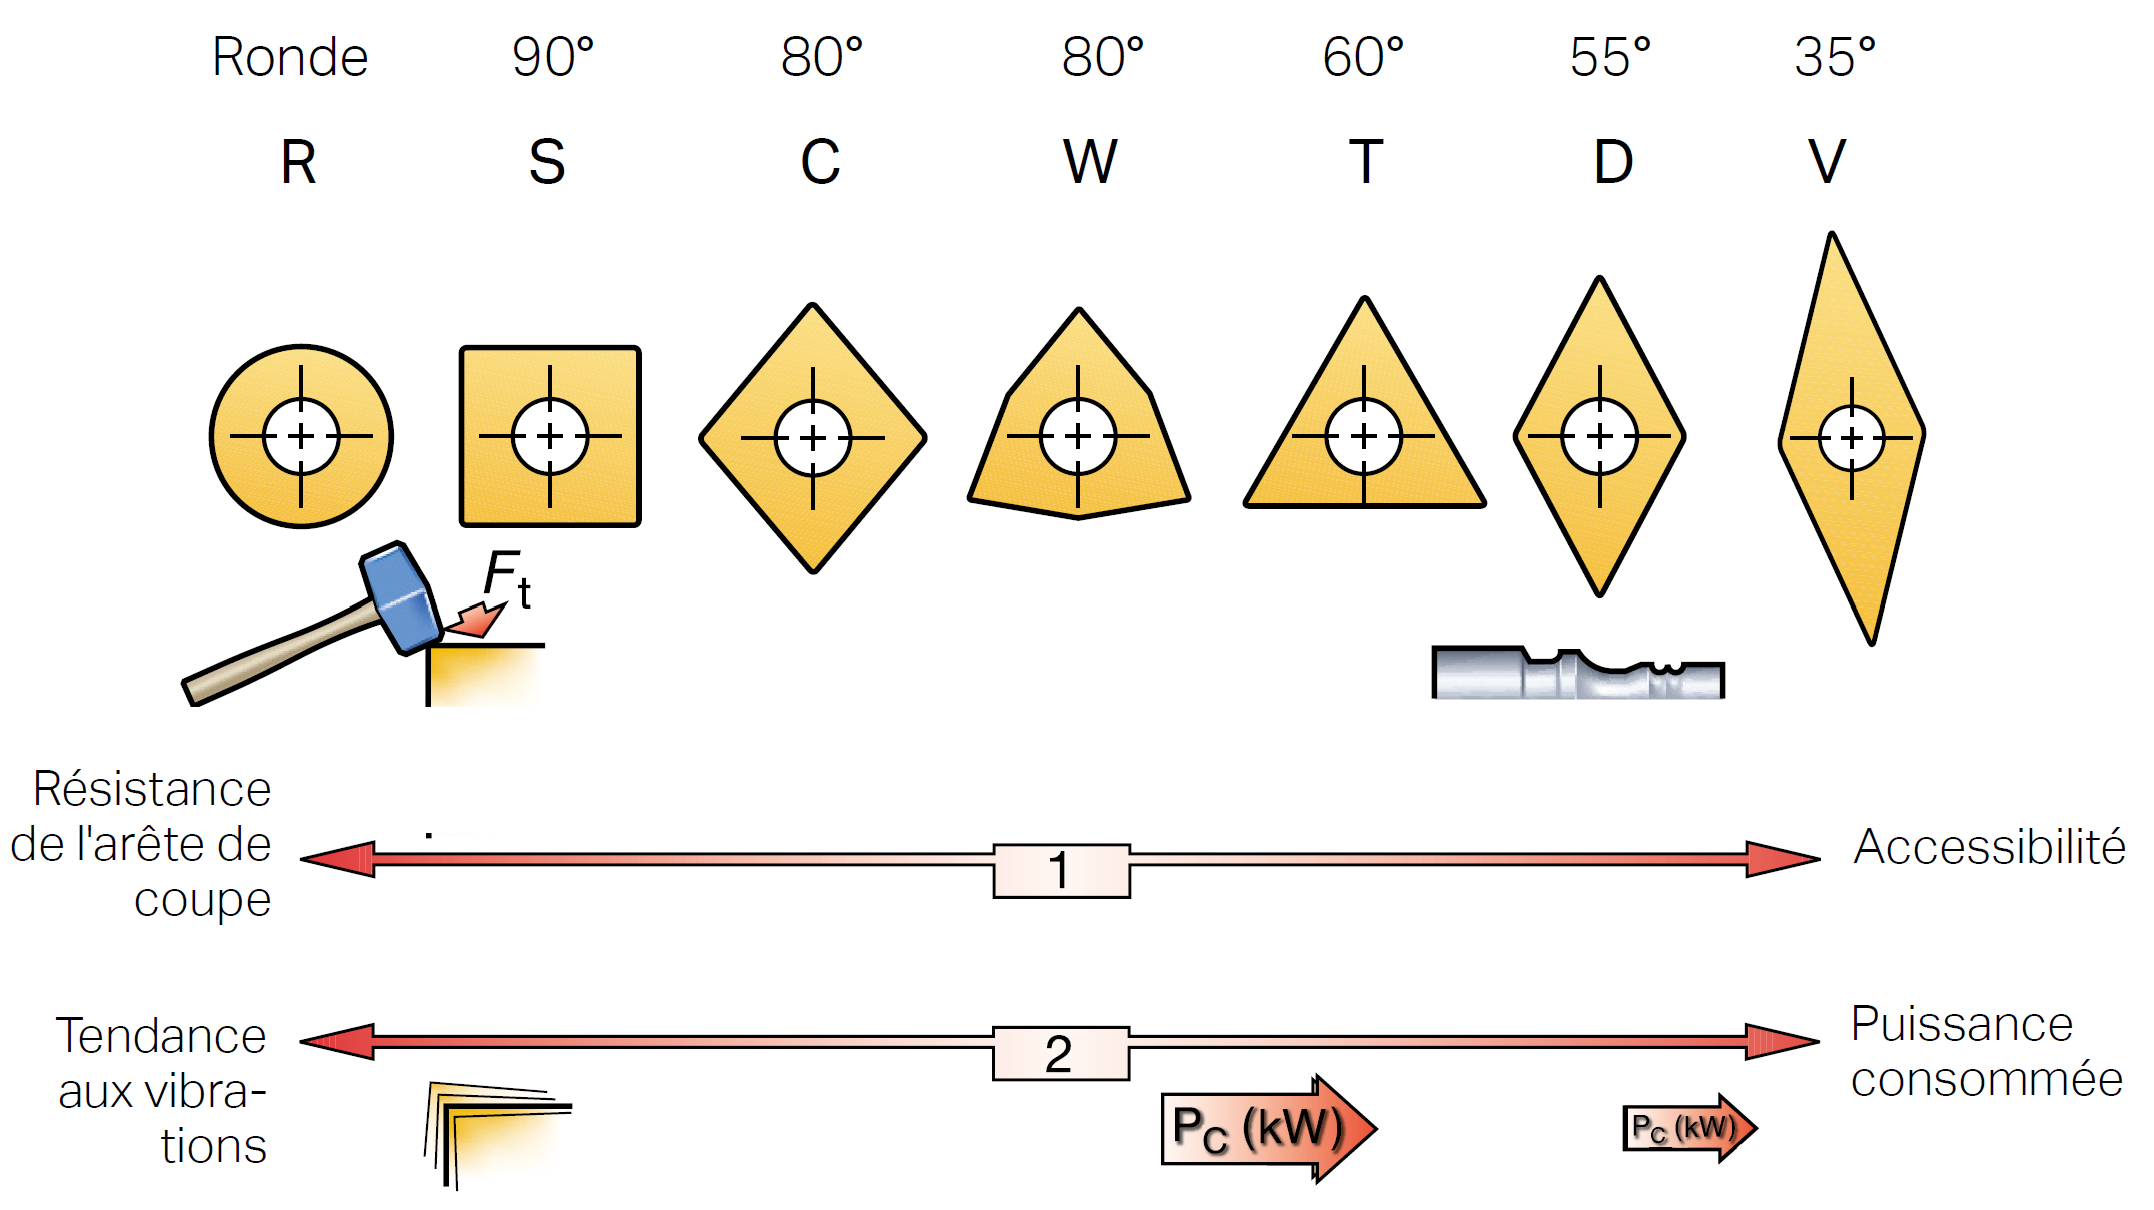
\includegraphics[width=0.85\linewidth]{CORR6.png}
\end{center}



\subsection{Application}
\begin{tcolorbox}[colback=blue!5!white,colframe=red!75!black]
   \bcdodecaedre Dans un atelier de production, le cahier des charges ainsi que la pièce demandée requiert un porte outil avec les contraintes suivantes :

\begin{itemize}
\item Fixation par bride et trou central ;
\item Plaquette Rhombique $80^{\circ}$;
\item Un angle d'attaque de $95^{\circ}$ par $95^{\circ}$;
\item Un angle de dépouille de $0^{\circ}$;
\item Une direction de coupe de gauche a droite ;
\item 25 mm de cote pour le corps du porte plaquette (plaquette carrée) ;
\item Un longueur de plaquette de 150 mm;
\item Une longueur de l'arrête de coupe de 12 mm.
\end{itemize}
  
\end{tcolorbox}
\begin{exo} En vous aidant des livres de production, trouver le porte plaquette idéal pour les besoins de l'atelier en donnant la codification de la plaquette sur la signalisation. \end{exo}

\marginnote{0,25 pt x 9 \\ = 2,25 pts}

\begin{center}
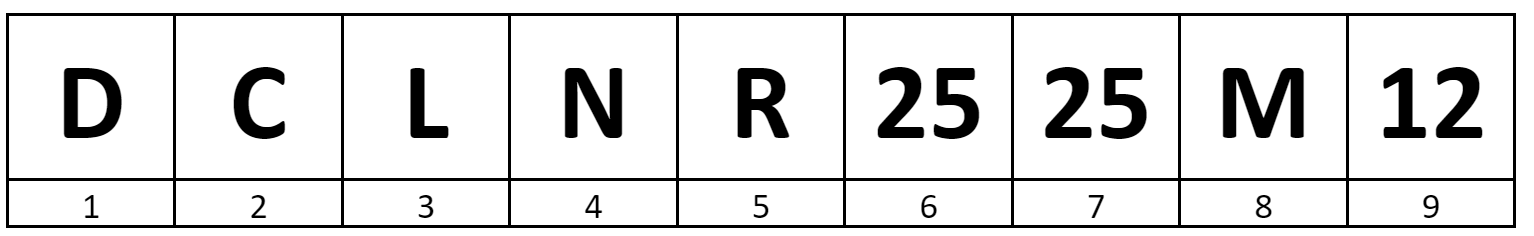
\includegraphics[width=0.85\linewidth]{CORR7.png}
\end{center}

\begin{tcolorbox}[colback=blue!5!white,colframe=red!75!black]
   \bcdodecaedre On vous informe que le porte plaquette que vous venez de choisir accueillera la plaquette suivante :
\begin{center}
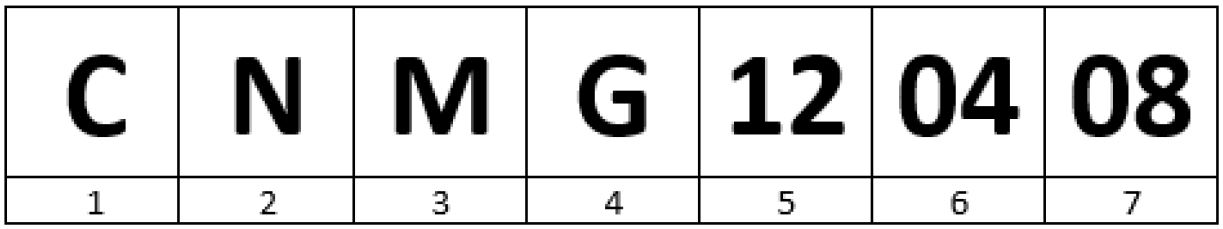
\includegraphics[width=0.7\linewidth]{PLA26.JPG}
\end{center}   
  
\end{tcolorbox}


\begin{exo} Indiquez la signification des 3 derniers numéros dans la codification des plaquettes de tournage métrique. \end{exo}

\marginnote{0,25 x 3 = 0,75 pt}

\textcolor{red}{5 : Taille de la plaquette (mm) ; \\ 6 : Épaisseur de la plaquette (mm) ; \\ 7 : Rayon de bec ($r^{\epsilon}$ en mm).}



\begin{exo} Quel(s) lien(s) pouvez-vous faire entre la signalétique du porte plaquette et la signalétique de la plaquette ?\end{exo}

\marginnote{0,5 pt}
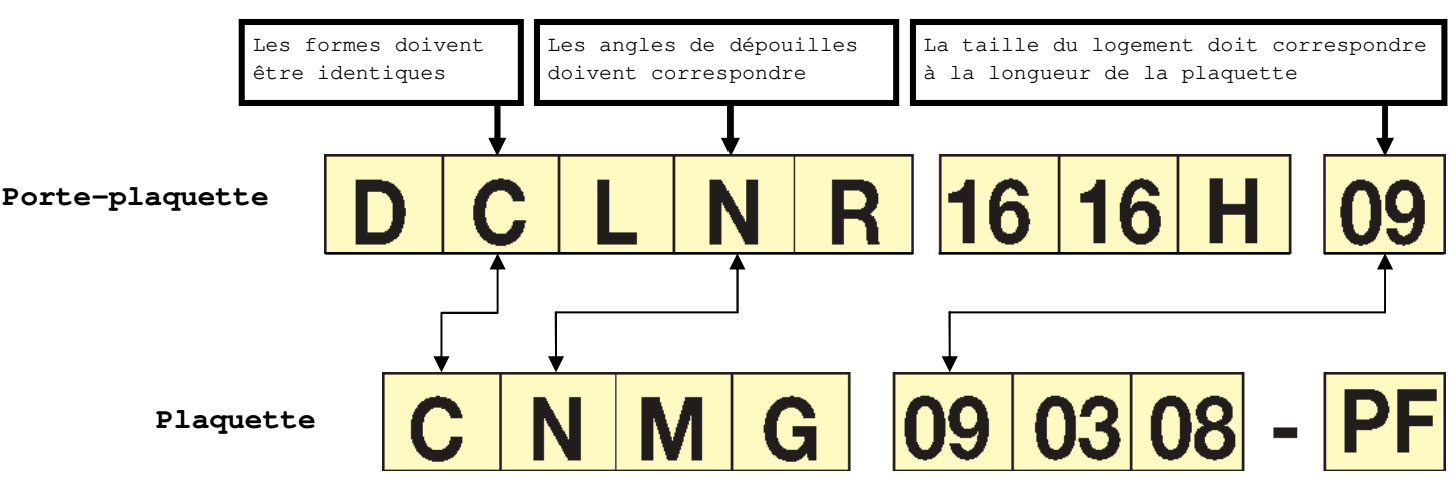
\includegraphics[width=0.95\linewidth]{CORR8.png}




\begin{tcolorbox}[colback=blue!5!white,colframe=red!75!black]
   \bcdodecaedre Vous êtes chargé de la sélection des outils (et si nécessaire de leur plaquette) de la gamme d'usinage suivantes :
\begin{center}
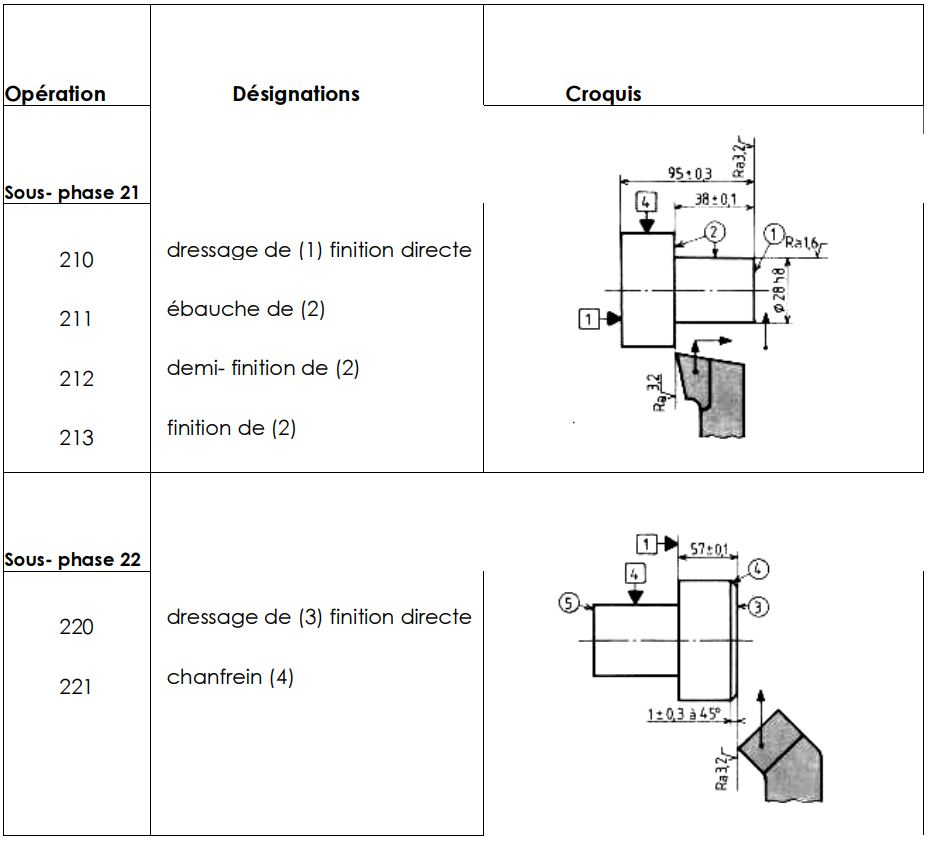
\includegraphics[width=0.75\linewidth]{G1.JPG}
\end{center}   
  \end{tcolorbox}


  \begin{exo} Sélectionnez l'outil, le porte outil et la plaquette si nécessaire pour les deux opérations suivantes :
\begin{itemize}
    \item 210 [Finition]
    \item 211 [Ébauche]
\end{itemize}
\end{exo}


\marginnote{1 pt }
\begin{tikzpicture}
\draw (0,0) -- (0,4) ;
\draw (0,4) -- (15,4) ;
\draw (15,4) -- (15,0) ;
\draw (15,0) -- (0,0) ;

\draw (0.2,3.9) node [anchor=north west][inner sep=0.75pt]   [align=left] {Sous-phase 210 : (porte-outil - outil - plaquette choisi)};
\end{tikzpicture}  



\marginnote{1 pt}
\begin{tikzpicture}
\draw (0,0) -- (0,4) ;
\draw (0,4) -- (15,4) ;
\draw (15,4) -- (15,0) ;
\draw (15,0) -- (0,0) ;

\draw (0.2,3.9) node [anchor=north west][inner sep=0.75pt]   [align=left] {Sous-phase 211 : (porte-outil - outil - plaquette choisi)};
\end{tikzpicture} 


\newpage

\subsection{Lubrification}

\begin{exo} Quels peuvent être les deux intérêts principaux de l'utilisation d'une lubrification interne ou externe ? Comparez les deux technologies.\end{exo}
\begin{center}
    \textbf{Lubrification EXTERNE}
\end{center}

\textcolor{red}{Avantage : Prix.} \\

\marginnote{1,25 pt}
\textcolor{red}{Inconvénients : Précision, débit du fluide.}

\begin{center}
    \textbf{Lubrification INTERNE}
\end{center}

\textcolor{red}{Avantage :  Précision, débit du fluide, topologie des canaux optimisés pour avoir moins de frottement, donc un bilan de consommation électrique meilleure} \\

\marginnote{1,25 pt}
\textcolor{red}{Inconvénients : Prix}







\begin{center}
    \textbf{FIN DU TP}
\end{center}



%----------------------------------------------------------------------------------------

\end{document}